\documentclass[10pt]{article}

% Lines beginning with the percent sign are comments
% This file has been commented to help you understand more about LaTeX

% DO NOT EDIT THE LINES BETWEEN THE TWO LONG HORIZONTAL LINES

%---------------------------------------------------------------------------------------------------------

% Packages add extra functionality.
\usepackage{times,graphicx,epstopdf,fancyhdr,amsfonts,amsthm,amsmath,algorithm,algorithmic,xspace,hyperref}
\usepackage[left=1in,top=1in,right=1in,bottom=1in]{geometry}
\usepackage{sect sty}	%For centering section headings
\usepackage{enumerate}	%Allows more labeling options for enumerate environments 
\usepackage{epsfig}
\usepackage[space]{grffile}
\usepackage{booktabs}
\usepackage{forest}
\usepackage{enumitem}   
\usepackage{fancyvrb}
\usepackage{todonotes}
\usepackage{array}

% This will set LaTeX to look for figures in the same directory as the .tex file
\graphicspath{.} % The dot means current directory.

\pagestyle{fancy}

\lhead{Final Project}
\rhead{\today}
\lfoot{CSCI 334: Principles of Programming Languages}
\cfoot{\thepage}
\rfoot{Spring 2024}

% Some commands for changing header and footer format
\renewcommand{\headrulewidth}{0.4pt}
\renewcommand{\headwidth}{\textwidth}
\renewcommand{\footrulewidth}{0.4pt}

% These let you use common environments
\newtheorem{claim}{Claim}
\newtheorem{definition}{Definition}
\newtheorem{theorem}{Theorem}
\newtheorem{lemma}{Lemma}
\newtheorem{observation}{Observation}
\newtheorem{question}{Question}

\setlength{\parindent}{0cm}

%---------------------------------------------------------------------------------------------------------

% DON'T CHANGE ANYTHING ABOVE HERE

% Edit below as instructed

\title{frisBRO Language Specification} % Replace SnappyLanguageName with your project's name

\author{Skylar Yarter \and Jocelyn Bliven} % Replace these with real partner names.

\begin{document}
  
\maketitle

\subsection*{Introduction}

\todo[inline]{This language helps a user decide what ultimate frisbee play to call in a given situation. When you are in the heat of the game, it can be hard to figure out what play to call. No longer! This programming language will help you decide what plays to call at any given moment based on where the players, disc, and the defensive force are. 
~\\
~\\
Ultimate frisbee requires “reading” the field to figure out what play is best to call and this reading of the field requires evaluating multiple parameters. A language that allows the user to read the field more easily and without human emotion and bias swaying the result would allow more appropriate plays to be called. Many of the evaluations being made by the players or coaches when choosing a play are quantitative (ie. where are the players and disc on the field, which way is the defense forcing). These quantitative parameters fit well within the scope of a programming language and can be compared better by a computer than a person standing on the field with a skewed perspective.
}

\subsection*{Design Principles}

\todo[inline]{We aim to create an easily readable, quick-to-type programming language so it can be used by frisbee coaches and players, who may not be familiar with general programming practices. Therefore, we prioritize simplicity in the syntax of our language so that it is easy to learn and to read. We do not want to overcomplicate the language by adding too many elements or rules, as that would hinder our user base. The language need not be object-oriented or follow a complex model as it is fairly basic, which allows for the easy-to-learn syntax.}

\subsection*{Examples}


    (Our syntax for our examples changed but for the most part, the underlying goal of the examples was accomplished)
    ~\\
    ~\\
    Example 1: Basic.txt
    ~\\
    Offense = \{(120,390), true; (140,220), false; (160,220), false; (180,220), false; (200,220), false; (220,220), false; (240,220), false; \}
    ~\\
    Defense = \{(120,370); (140,200); (160,200); (180,200); (200,200); (220,200); (240,200); \}
    ~\\
    Defense = Manual
    ~\\
    Force = Home
    ~\\
    ~\\
   
    ~\\
    ~\\
    Example 2: Automatic Person Defense (auto.txt)
    ~\\
    Offense = \{(220,390), true; (220,220), false; (300,220), false; (320,220), false; (340,220), false; (360,220), false; (380,220), false; \}
    ~\\
    Defense = Automatic
    ~\\
    Force = Away
    ~\\
    ~\\

    ~\\
    ~\\
    Example 3: Endzone
    ~\\
    Offense = \{(220,390), true; (220,270), false; (220,140), false; (400,350), false; (400,275), false; (400,175), false; (400,100), false; \}
    ~\\
    Defense = Automatic
    ~\\
    Force = Home
    ~\\
    Play = if disc in range 100 to 300 and force is Force = Home
    ~\\
    ~\\
    



Example 1 Output: 
\begin{center}
    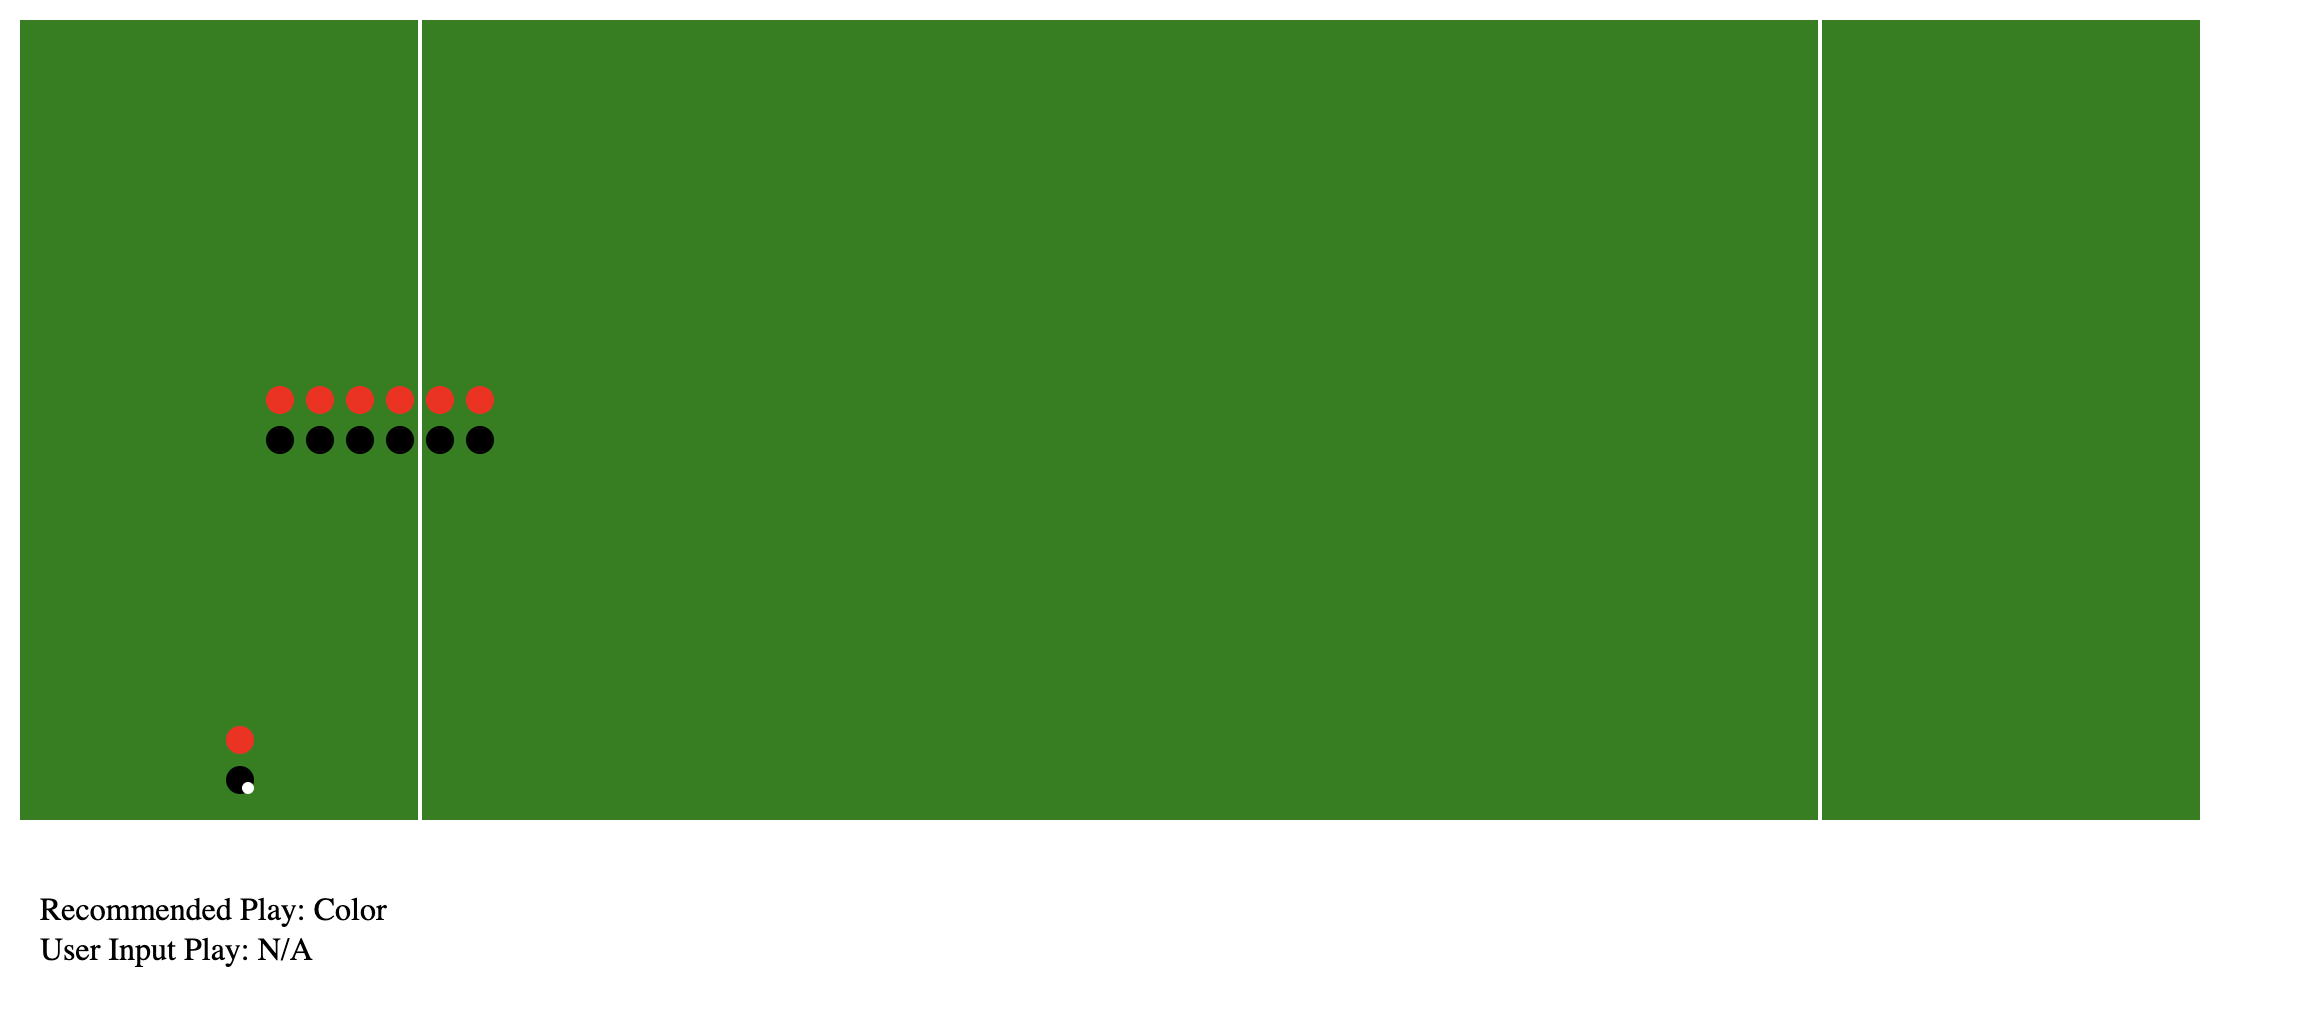
\includegraphics[width=.8\textwidth]{images/basic.png}
\end{center}

Example 2 Output: 
\begin{center}
    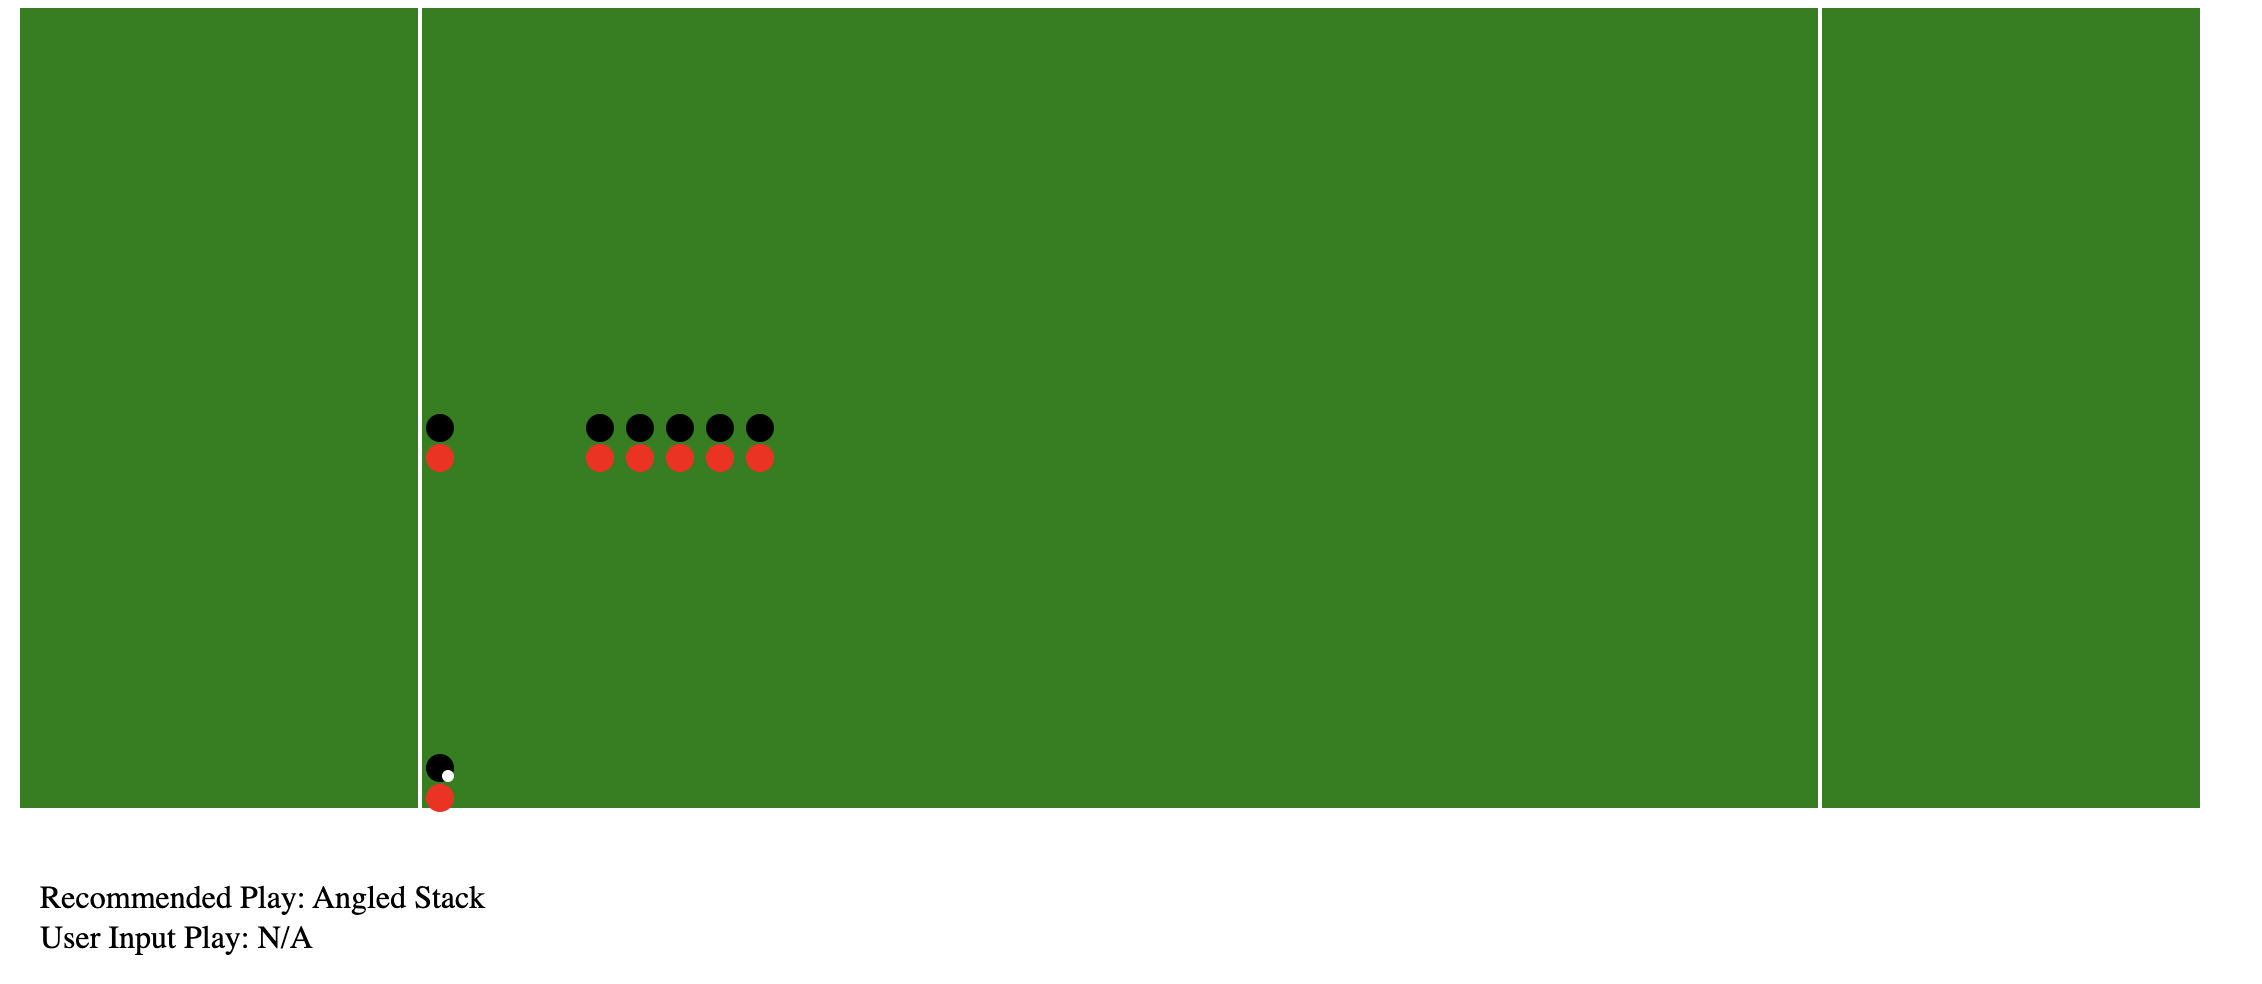
\includegraphics[width=.8\textwidth]{images/auto.png}
\end{center}

Example 3 Output: 
    \begin{center}
        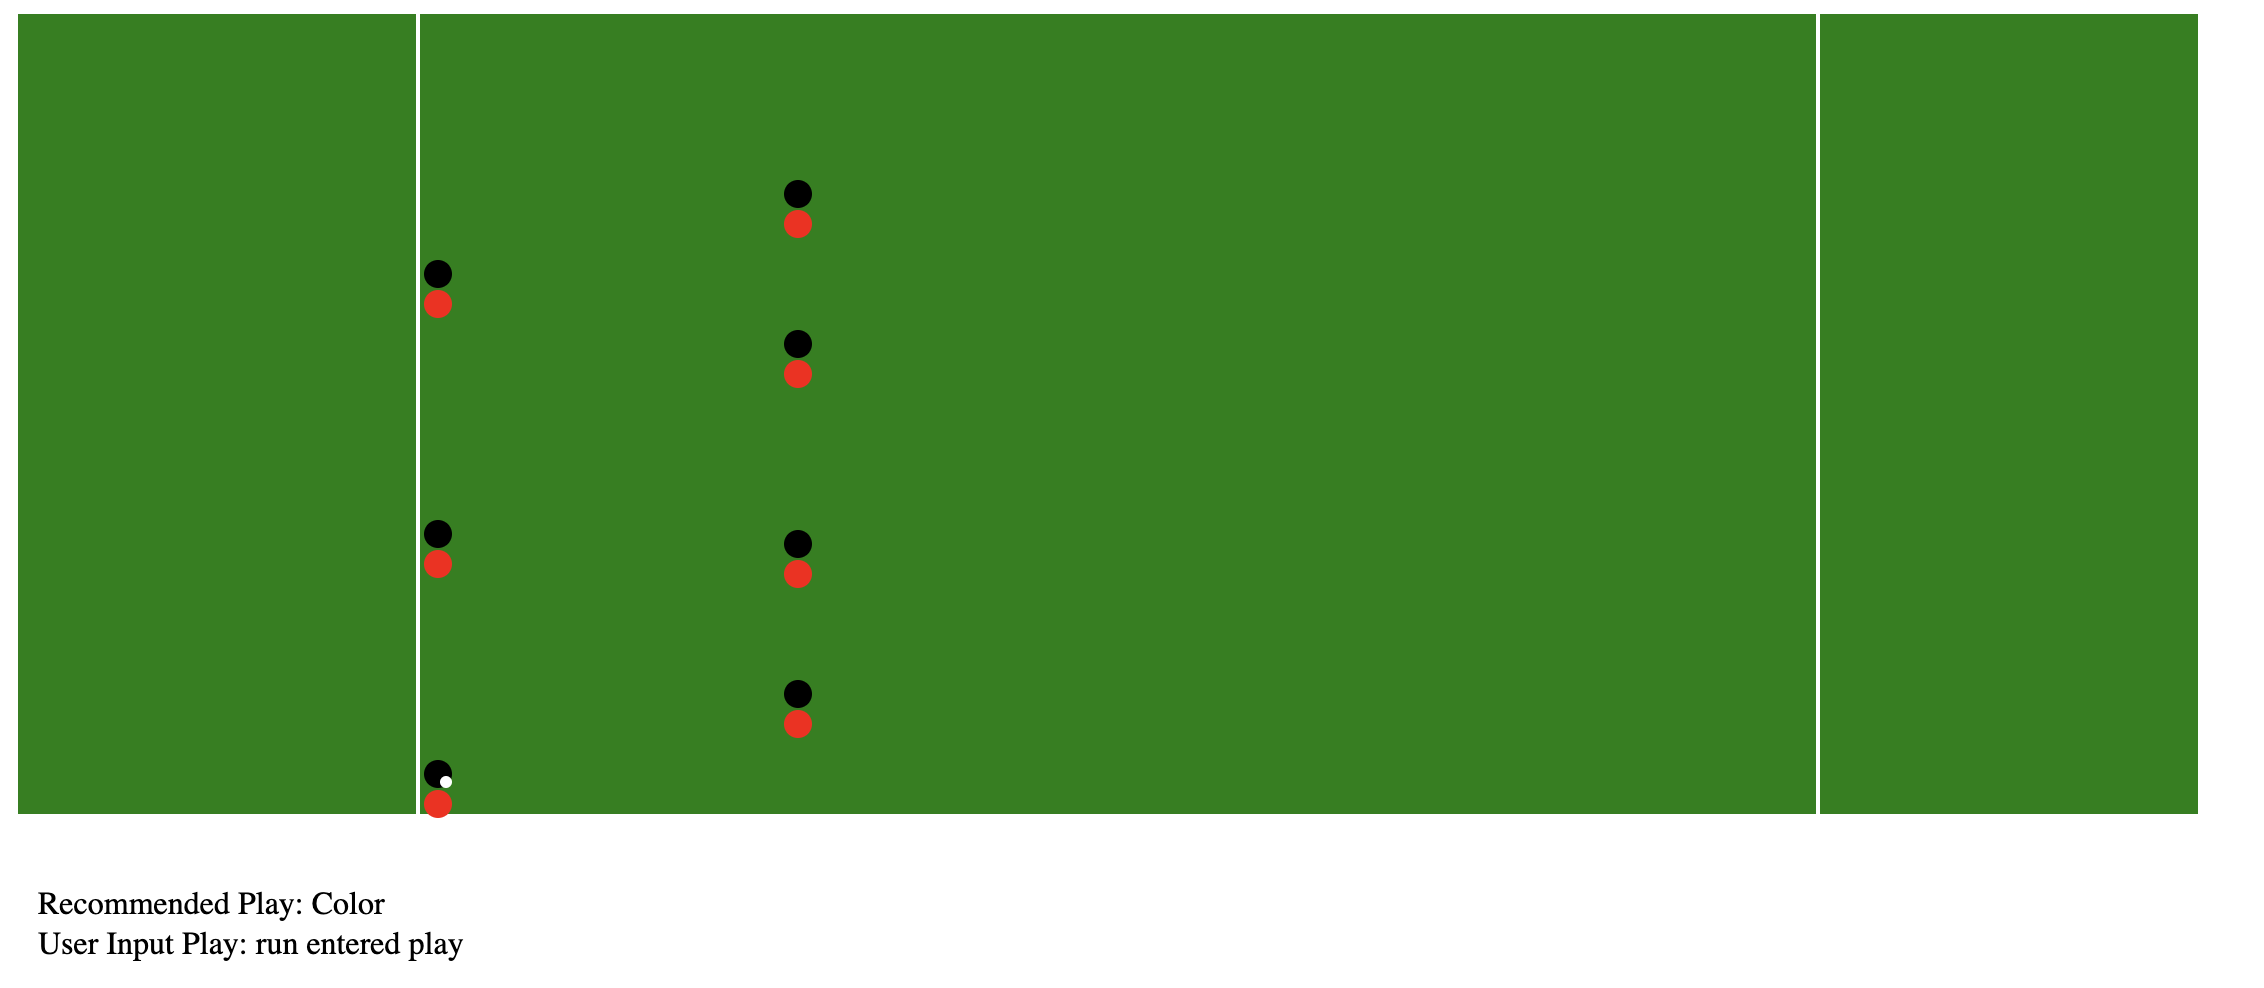
\includegraphics[width=.8\textwidth]{images/addedplay.png}
    \end{center}

\subsection*{Language Concepts}

\todo[inline]{A user needs to understand that each offensive and defensive player is a unique object which is essentially just a coordinate. The primitives of this language are coordinates which ultimately determine where the players and the disc are. The multiple players are combined into a team. Other primitives are the defensive force which is basically just a string. Adding the force and where the disc is allows the user to fine-tune what play they should call. The field is a combining form which takes all the teams, disc, and force and places them in the correct position. Additionally, the user should understand how the field is set up and how to visualize it.}

Field Visualization: 
\begin{center}
    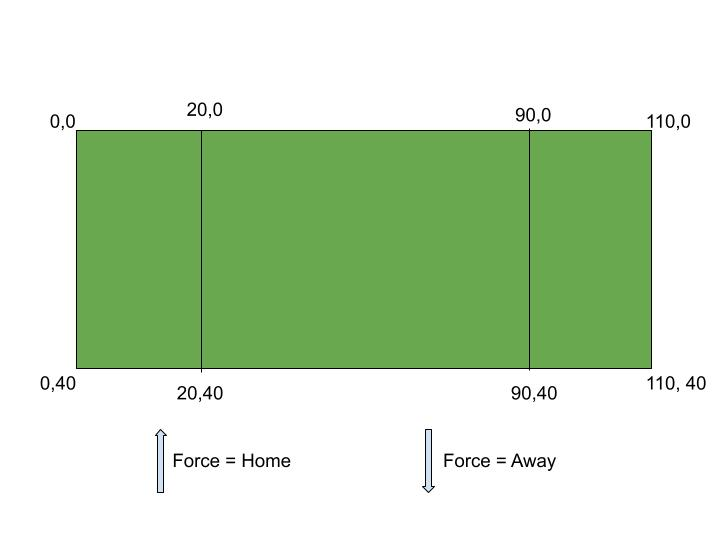
\includegraphics[width=.5\textwidth]{images/FieldVisualization.jpg}
\end{center}

\subsection*{Formal Syntax}

\todo[inline]{ 
% Current syntax:
% ~\\
%     $<$expr$>$		::=$<$offense$>$$<$defense$>$
%     ~\\
%     $<$offense$>$	::= $<$oplayer$>$$<$offense$>$ $|$ $<$oplayer$>$
%     ~\\
%     $<$defense$>$	::= $<$dplayer$>$$<$defense$>$ $|$ $<$dplayer$>$
%     ~\\
    
%     $<$oplayer$>$ 	::= $<$coordinate$>$$<$disc$>$
%     ~\\
%     $<$dplayer$>$	::= $<$coordinate$>$
%     ~\\
%     $<$disc$>$  	::= true $|$ false
%     ~\\
%     $<$coordinate$>$::= ($<$digit$>$,$<$digit$>$)
%     ~\\
%     $<$digit$>$		    ::= $<$digit$>$n $|$ n  where n is any positive integer
% ~\\
% ~\\
Syntax: 
~\\
    $<$expr$>$		::= $<$field$>$$<$plays$>$ $|$ $<$field$>$
    ~\\
    $<$field$>$		::=$<$teams$>$$<$flag$>$$<$force$>$
    ~\\
    $<$teams$>$     ::= $<$offense$>$ | $<$offense$>$$<$defense$>$
    ~\\
    $<$offense$>$	::= $<$oplayer$>$$<$offense$>$ $|$ $<$oplayer$>$
    ~\\
    $<$defense$>$	::= $<$dplayer$>$$<$defense$>$ $|$ $<$dplayer$>$  
    ~\\
    $<$hasdisc$>$  	::= true $|$ false
    ~\\
    $<$oplayer$>$ 	::= $<$coordinate$>$$<$hasdisc$>$
    ~\\
    $<$dplayer$>$	::= $<$coordinate$>$
    ~\\
    $<$force$>$ 	::= home $|$ away $|$ flat
    ~\\
    $<$flag$>$      ::= automatic $|$ manual
    ~\\
    $<$plays$>$ 	::= $<$play$>$ $|$ $<$play$>$$<$plays$>$ $|$ Library
    ~\\
    $<$play$>$ 		::= if disc in range $<$digit$>$ to $<$digit$>$ and force is Force = $<$force$>$ with name as $<$playname$>$
    ~\\
    $<$playname$>$  ::= string
    ~\\
    $<$coordinate$>$::= ($<$digit$>$,$<$digit$>$)
    ~\\
    $<$digit$>$		    ::= $<$digit$>$n $|$ n  where n is any positive integer

}

\subsection*{Semantics}

\todo[inline]{The primitives in this language are coordinates, defense types, booleans, and the force. Plays are programs passed in or accessed in a Library as strings.
~\\
~\\
The combining forms in this language are players, which are made from coordinates and booleans determining if they have the disc; teams, which are made of lists of players; and a field, which is made from combining teams and the force on the field.
~\\
~\\
The programs in our language can optionally read in a file containing a team’s plays. The plays would be written in with booleans to indicate when to use them (e.g., “if force=home, then angled stack”). If the user does not provide a file of plays, the program will use the default plays that we provide.
~\\
~\\
In its simplest state, the output of a program will be a frisbee field with the players and disc at the correct coordinates. For our final version of the language, the output of a program will be a picture of the field with a list of suggested plays, either from the library or from the user’s inputted plays.

}


\begin{center}
    \begin{tabular}{ | m{5cm} | m{5cm}|  m{5cm} |} 
      \hline
      Syntax & Abstract Syntax & Meaning \\ 
      \hline
      $<$n$>$ & Digit of int & n is a primative integer stored using F\# integers \\
      \hline
      ($<$n$>$,$<$n$>$) & Coordinate of {x: int; y: int} & x and y are integers. A coordinate is a primitive that represents where on the field a player is. \\ 
      \hline
      $<$coordinate$>$, $<$hasDisc$>$ & Offense of Coordinate * HasDisc & An offensive player is made up of a coordinate and a boolean value of whether or not they have the disc. The player is drawn on the field in the appropriate location with/without the disc based on this information. \\ 
      \hline
      $<$coordinate$>$ & Defense of Coordinate & A defensive player is made up of a coordinate. The player is drawn on the field in the appropriate location. \\ 
      \hline
      $<$coordinate$>$, $<$hasDisc$>$ $|$ $<$coordinate$>$ & Offense of Coordinate * HasDisc or Defense of Coordinate & A player is either on Offense or Defense. Players are used to create Teams which are a list of players\\
      \hline
      ($<$player$>$, $<$offensive$>$) $|$ $<$player$>$ & Offensive of Player list & Offensive (which symbolizes an offensive team) is a list of offensive players. This is a combining form of offensive players. \\
      \hline
      ($<$player$>$, $<$defensive$>$) $|$ $<$player$>$ & Defense of Player list & Offensive (which symbolizes an offensive team) is a list of offensive players. This is a combining form of offensive players. \\
      \hline
      True $|$ False & HasDisc of True or False & Determines if offensive player has a disc \\
      \hline
      Automatic $|$ Manual & Flag of Automatic or Manual & Determines if user put in their own defense or not \\
      \hline
      Home $|$ Away $|$ Flat & Force of Home or Away or Flat & Tells the program what the force is on the feild \\
      \hline
      if disc in range $<$n$>$ to $<$n$>$ and force = $<$force$>$ with name as $<$name$>$ & Play of (int * int) * Force * Name & User inputed play that allows the user to determine if they want to run a play based on a range and a force. \\
      \hline
      Offense = $<$Offensive$>$ Defense = $<$defensive$>$ Force = $<$force$>$ Play = $<$plays$>$ & Field of Team list * Flag * Force * Play list & The final combining form which collects all user input into a usable tuple \\
      \hline
    \end{tabular}
\end{center}

\subsection*{Remaining Work}

While we believe that this language would help ultimate frisbee players in this current
itteration some improvements could be made to increase functionality. First of all arrows which 
point to where players should run could be added to the out put such that the user and their team
would be able to clearly see how running the suggesested play would end up. Secondly,
the language could be updated to allow for more detail in the user entered plays. For example, 
the user could specify where the disc is on the field horizontally, not just vertically. 

% DO NOT DELETE ANYTHING BELOW THIS LINE
\end{document}
